\documentclass[12pt]{article}
\usepackage{fullpage}
\usepackage{float}
\usepackage{graphicx}
\usepackage{subcaption}
\usepackage{amsmath}
\usepackage{amsfonts}
\usepackage{amssymb}
\usepackage{algpseudocode}
\usepackage{algorithm}


\begin{document}
\title{Notes on Domain Decomposition}
\author{Scott Aiton}
\maketitle

\section{Forming Schur Complement Matrix}

If there is a $\gamma$ for each point on the interface, how to we determine the values?
\begin{figure}[H]
    \centering
    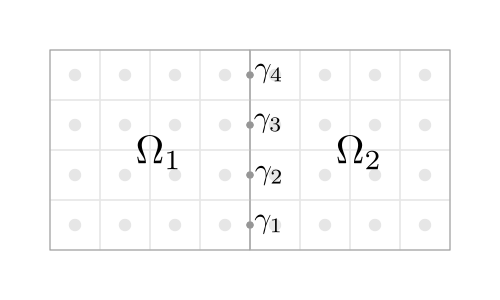
\includegraphics[width=4in]{images/abdomain.pdf}
    \caption{Two domain example}
\end{figure}
We want the gamma value to equal to the average of the solution on both sides:
\begin{equation}
    \gamma = \frac{East(\Omega_1)+West(\Omega_2)}{2}
\end{equation}
Where $East$ and $West$ are subroutines that return the solution values along the east side or west side
of a domain.
So now we have a function of $\gamma$
\begin{equation}
    F(\gamma)=2\gamma-(East(\Omega_1)+West(\Omega_2))
    \label{function}
\end{equation}
that we want to find the zero of. In subroutine form, this would look like:
\begin{algorithm}[H]
\caption{Two-Domain Function}
\begin{algorithmic}[1]
    \Procedure{F}{$\gamma$}
    \State $\Omega_1.solveWithInterface(\gamma)$
    \State $\Omega_2.solveWithInterface(\gamma)$
    \State \Return $2\gamma-(East(\Omega_1)+West(\Omega_1))$
    \EndProcedure
\end{algorithmic}
\end{algorithm}

When there are multiple interface points, then we have a system of linear equations
\begin{equation}
F(\gamma)=A\gamma-b
\end{equation}
The $b$ vector is found by
\begin{equation}
b=-F(0)
    \label{bvec}
\end{equation}
and each column of the matrix is found by
\begin{equation}
A(:,i) = F(e_i)+b
    \label{matrixcol}
\end{equation}
we can then determine the  $\gamma$ vector by solving
\begin{equation}
A\gamma=b
\end{equation}
\subsection{Generalized Function}
\begin{algorithm}[H]
\caption{Generalized Function}
\begin{algorithmic}[1]
    \Procedure{F}{$\gamma, Domains$}
    \State $result(\gamma.size())$ \Comment{Allocate new vector}
    \For{$\Omega \in Domains$}
        \State $\Omega.solveWithInterface(\gamma)$
        \For{$side \in \{North,East,South,West\}$}
            \If{$\Omega.hasNeighbor(side)$}
                \State $i \gets \Omega.ifaceIndex(side)$
                \State $start \gets i*n$
                \State $stop \gets (i+1)*n$
                \State $result(start:stop) \gets \gamma(start:stop) - \Omega.getSolutionEdge(side)$
            \EndIf
        \EndFor
    \EndFor
    \State \Return $result$
    \EndProcedure
\end{algorithmic}
\end{algorithm}

\section{Quick Formation of the Schur Complement Matrix}
In this section, we can use the process described in equation \eqref{matrixcol} to derive an algorithm
that allow us to quickly form the Schur compliment matrix.
\paragraph{The matrix does not depent on the RHS on the domains}
First, let's reconsider equations  \eqref{bvec} and \eqref{matrixcol}. If we are solving on a system
where the rhs and lhs on each patch is zero, the $b$ vector for the Schur complement matrix will
be $0$, since $0$ is the correct solution for the interfaces. So equation \ref{matrixcol} turns into
\begin{equation}
    A(:,i) = F_{zero}(e_i)
\end{equation}
where $F_{zero}$ is the same as equation \ref{function} but with the rhs on each domain replaced 
with $0$.
So now we use can use this to reduce the amount of work needed to form the Schur complement matrix.
\\
\\
Let's consider what happens when we solve for $F_{zero}(e_i)$. If a single interface value is set
to $1$, only the two adjacent domains will have non-zero dirichlet boundary conditions, meaning that
only the two adjacent domains will have non-zero solutions. This means that when we are solving for 
$F_{zero}(e_i)$, we can  assume that solution on any domain that is not adjacent to the interface
with the $1$ is zero. In other words, we only have to do a solve on the two adjacent domains, rather
than solving for all the domains.

\paragraph{Indexing of $\gamma$ Values} 
If the individual values in the $\gamma$ vector are indexed in the following way:
\begin{itemize}
    \item If the interface is on the east or west side of the patch, the $\gamma$ values will be indexed consecutively from the bottom up.
    \item If the interface is on the north or south side of the patch, the $\gamma$ values will be indexed consecutively from left to right.
\end{itemize}
\begin{figure}[H]
    \centering
    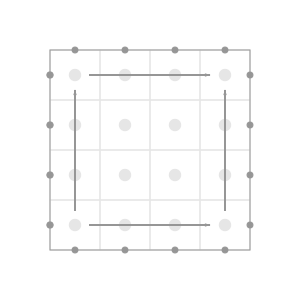
\includegraphics[width=3in]{images/indexing.pdf}
    \caption{Indexing of $\gamma$ values}
\end{figure}
Since the $\gamma$ values on each interface indexed consecutively, the Schur complement matrix takes
on a block structure, where each block is $n\times n$.
\paragraph{Sparsity}

Consider the example grid given in Figure \ref{2domain}.
When a single $1$ is set on the interface $i_{\textnormal{main}}$, only 7 interfaces will end up
having non-zero values: the main interface, $i_{\textnormal{main}}$, and the 6 auxiliary
interfaces, 
$i_{\textnormal{left north}}$, $i_{\textnormal{left south}}$, $i_{\textnormal{left west}}$,
$i_{\textnormal{right north}}$, $i_{\textnormal{right east}}$, and $i_{\textnormal{right south}}$.

\begin{figure}[H]
    \centering
    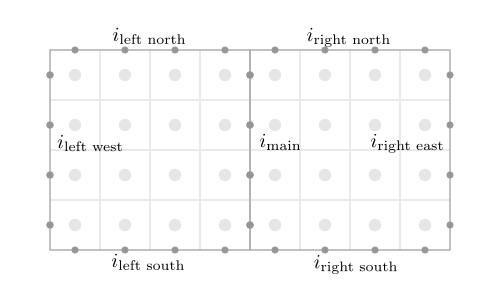
\includegraphics[width=6in]{images/2domain.pdf}
    \caption{Two domain example}
    \label{2domain}
\end{figure}

\paragraph{Splitting up the work}

If we look at equation \ref{function}, we can split up the work and process the two domains at
different times.
\begin{align}
    F_{left}(\gamma)&=\gamma-L(\gamma) \label{function_left}\\
    F_{right}(\gamma)&=\gamma-R(\gamma) \label{function_right}
\end{align}

So, when we process the left and right domains, we use equations \eqref{function_left} and 
\eqref{function_right}, respectively, for the diagonal blocks ($i_{\textnormal{main}}$).
When we are forming the matrix, we will insert the diagonal
block twice, summing the coefficients of one block into the other.

\paragraph{Rotation}
\begin{figure}
    \centering
    \begin{subfigure}[b]{0.30\textwidth}
        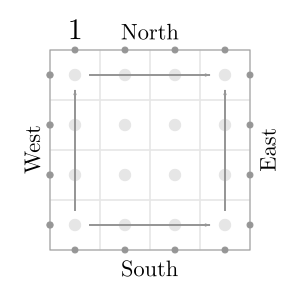
\includegraphics[width=\textwidth]{images/north1.pdf}
        \caption{North}
    \end{subfigure}
    \begin{subfigure}[b]{0.30\textwidth}
        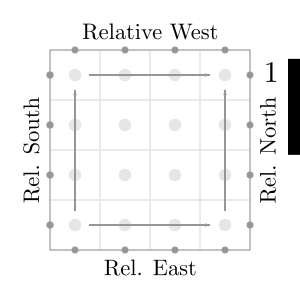
\includegraphics[width=\textwidth]{images/east1.pdf}
        \caption{East}
    \end{subfigure}
    \begin{subfigure}[b]{0.30\textwidth}
        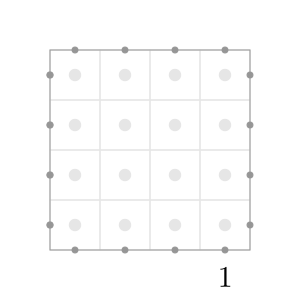
\includegraphics[width=\textwidth]{images/south1.pdf}
        \caption{South}
    \end{subfigure}
    \begin{subfigure}[b]{0.30\textwidth}
        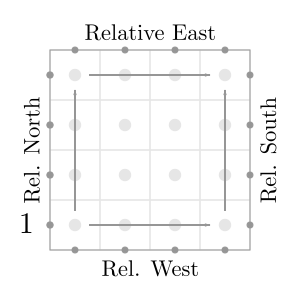
\includegraphics[width=\textwidth]{images/west1.pdf}
        \caption{West}
    \end{subfigure}

    \caption{Rotation}
    \label{rotation}
\end{figure}

We can get the coefficients for the blocks in the Schur complement matrix by
setting each $\gamma$ value along one side of the domain to $1$, and then reuse these coefficients 
for the interfaces on the other sides.

Let the north side be our canonical side. If we set each $\gamma$ value along the north interface to
$1$, we can save the resulting coefficients into four blocks. This is done in algorithm
\ref{getblocks}.

Let's consider part (a) in figure \ref{rotation} where the
first $\gamma$ value on the north interface is set to $1$. If rotate this domain clockwise by $90$
degrees, that is equivalent to setting the last $\gamma$ value on the east interface to $1$. If we
rotate it again, it is equivalent to setting the last $\gamma$ value on the south interface to
$1$. And if we rotate once more, it would be equivalent to setting the first $\gamma$ value on the
east interface. What this means is that if we want to reuse the blocks from the north interface 
for either the east or south interface, we will have to reverse the order of the columns in the 
blocks.

Another thing that we will have to consider is that order of the rows for the canonical east and
west blocks will also have to be reversed if we are using them on either the south or west
interfaces. To illustrate this, let's look at the south interface on figure \ref{rotation}. When we
are solving along the north interface, the arrows along east and west of the domain are pointing
towards the interface. But when we look at the south interface, the arrows are pointing away from
it. This means that when we are 


\begin{algorithm}
\caption{}
\label{getblocks}
\begin{algorithmic}[1]
    \Procedure{getBlocks}{n}
    \State $\Omega()$ \Comment{Create empty domain}
    \State $\Omega.rhs \gets 0$
    \State $\Omega.northBoundary \gets 0$
    \State $\Omega.eastBoundary \gets 0$
    \State $\Omega.southBoundary \gets 0$
    \State $\Omega.westBoundary \gets 0$
    \State $NorthBlock(n*n)$ \Comment{Allocate blocks of size n*n}
    \State $EastBlock(n*n)$
    \State $SouthBlock(n*n)$
    \State $WestBlock(n*n)$
    \For{$i \gets 1,n$}
         \State $\Omega.northBoundary(i) \gets 1$
         \State $\Omega.\Call{solve}{ }$
         \State $NorthBlock(:,i) \gets \Omega.northBoundary - \Call{North}{\Omega}$
         \State $EastBlock(:,i) \gets -\Call{East}{\Omega}$
         \State $SouthBlock(:,i) \gets -\Call{South}{\Omega}$
         \State $WestBlock(:,i) \gets -\Call{West}{\Omega}$
         \State $\Omega.northBoundary(i) \gets 0$
    \EndFor

    \State \Return $NorthBlock, EastBlock, SouthBlock, WestBlock$
    \EndProcedure
\end{algorithmic}
\end{algorithm}
\paragraph{Algorithm}

%\begin{algorithm}
%\caption{Quick Schur Compliment Formation}
\begin{algorithm}[H]
\caption{}
\begin{algorithmic}[1]
    \Procedure{EnumerateIfaceStructs}{Domains}
    \State $ifaces \gets \emptyset$ \Comment{Set of interfaces to be processed}
    \ForAll{$\Omega \in Domains$}
        \If{$\Omega.northIndex \not= null$}
            \State $iface()$ \Comment{New iface object}
            \State $iface.side \gets North$
            \State $iface.northIndex \gets \Omega.northIndex$
            \State $iface.eastIndex \gets \Omega.eastIndex$
            \State $iface.southIndex \gets \Omega.southIndex$
            \State $iface.westIndex \gets \Omega.westIndex$
            \State $ifaces.insert(iface)$
        \EndIf
        \If{$\Omega.eastIndex \not= null$}
            \State $iface()$ \Comment{New iface object}
            \State $iface.side \gets East$
            \State $iface.northIndex \gets \Omega.eastIndex$
            \State $iface.eastIndex \gets \Omega.southIndex$
            \State $iface.southIndex \gets \Omega.westIndex$
            \State $iface.westIndex \gets \Omega.northIndex$
            \State $ifaces.insert(iface)$
        \EndIf
        \If{$\Omega.southIndex \not= null$}
            \State $iface()$ \Comment{New iface object}
            \State $iface.side \gets South$
            \State $iface.northIndex \gets \Omega.southIndex$
            \State $iface.eastIndex \gets \Omega.westIndex$
            \State $iface.southIndex \gets \Omega.northIndex$
            \State $iface.westIndex \gets \Omega.eastIndex$
            \State $ifaces.insert(iface)$
        \EndIf
        \If{$\Omega.westIndex \not= null$}
            \State $iface()$ \Comment{New iface object}
            \State $iface.side \gets West$
            \State $iface.northIndex \gets \Omega.westIndex$
            \State $iface.eastIndex \gets \Omega.northIndex$
            \State $iface.southIndex \gets \Omega.eastIndex$
            \State $iface.westIndex \gets \Omega.southIndex$
            \State $ifaces.insert(iface)$
        \EndIf
    \EndFor
    \State \Return $ifaces$
    \EndProcedure
\end{algorithmic}
\end{algorithm}
\begin{algorithm}[H]
\caption{Matrix Formation}
\begin{algorithmic}[1]
    \Procedure{FormMatrix}{Domains}
    \State $ifaces \gets \Call{EnumerateIfaceStructs}{Domains}$
    \State $NorthBlock, EastBlock, SouthBlock, WestBlock \gets \Call{getBlocks}{n}$
    \State $A()$ \Comment{Allocate Matrix}
    \ForAll{$iface \in ifaces$} \Comment{Insert Blocks into Matrix}
        \State $reverseColumns \gets False$
        \State $reverseRows \gets False$
        \If {iface.side = East \textbf{or} iface.side = South}
             \State $reverseColumns \gets True$
        \EndIf
        \State
        \State $j \gets iface.northIndex$
        \State $A.insertBlock(NorthBlock,j,j,reverseColumns,reverseRows)$
        \State
        \If{$\Omega.southIndex \not= null$}
            \State $i \gets iface.southIndex$
            \State $A.insertBlock(SouthBlock,i,j,reverseColumns,reverseRows)$
        \EndIf
        \State
        \If {iface.side = South \textbf{or} iface.side = West}
             \State $reverseRows \gets True$
        \EndIf
        \State
        \If{$\Omega.eastIndex \not= null$}
            \State $i \gets iface.eastIndex$
            \State $A.insertBlock(EastBlock,i,j,reverseColumns,reverseRows)$
        \EndIf
        \State
        \If{$\Omega.westIndex \not= null$}
            \State $i \gets iface.westIndex$
            \State $A.insertBlock(WestBlock,i,j,reverseColumns,reverseRows)$
        \EndIf
        \State
    \EndFor
    \EndProcedure
\end{algorithmic}
\end{algorithm}
%\end{algorithm}




\section{Handling Refinement}
We want the flux going out of the coarse cell to match the fluxes going into 
the fine cells.

\begin{figure}[H]
    \centering
    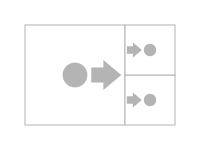
\includegraphics[width=4in]{images/amrflux.pdf}
    \caption{flux}
\end{figure}

We can represent this with the equation:

\begin{equation}
    \Phi_{c}=\Phi_{f_1}+\Phi_{f_2}
    \label{fluxconsv}
\end{equation}

\subsubsection*{Coming up with a stencil}
Lets say we want to find the ghost values for the coarse cell, the first fine cell, and the second
fine cell. Labeled $g_c$,$g_{f_1}$,and $g_{f_2}$, respectively.

\begin{figure}[H]
    \centering
    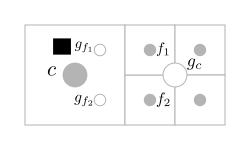
\includegraphics[width=4in]{images/ghost.pdf}
    \caption{ghost points}
\end{figure}

We can enforce flux conservation by interpolating to the fine ghost points, and then using equation
\ref{fluxconsv} to find the ghost point for the coarse cell.

The fluxes for each cell will be:
\begin{align}
    \Phi_c&=g_c-c\\
    \Phi_{f_1}&=f_1-g_{f_1}\\
    \Phi_{f_2}&=f_2-g_{f_2}
\end{align}

We can then solve for the value of $g_c$:

\begin{align}
    \Phi_{c}&=\Phi_{f_1}+\Phi_{f_2}\\
    g_c-c   &=f_1-g_{f_1}+f_2-g_{f_2}\\
    g_c     &=c+f_1-g_{f_1}+f_2-g_{f_2}
    \label{ghostconsv}
\end{align}

\subsubsection*{Bilinear interpolation}

Bilinear interpolation for the fine ghost points works, but error is not continuous.

TODO: Explain this and show an example

\subsubsection*{Quadratic interpolation}



\begin{figure}[H]
    \centering
    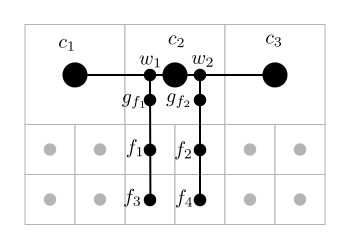
\includegraphics[width=5in]{images/quadstencil.pdf}
    \caption{flux}
\end{figure}

To find the value of $g_{f_1}$, we first use quadratic interpolation with the points 
$c_1$, $c_2$, and $c_3$ to interpolate to $w_1$:
\begin{equation*}
    w_1=\frac{5}{32}c_1+\frac{15}{16}c_2-\frac{3}{32}c_3
\end{equation*}
We then use quadratic interpolation with the points 
$w_1$, $f_1$, and $f_3$ to interpolate to $g_{f_1}$:
\begin{equation*}
    g_{f_1}=\frac{8}{15}w_1+\frac{2}{3}f_1-\frac{1}{5}f_3
\end{equation*}
Plug in the value for $w_2$, and we get the final equation for $g_{f_1}$:
\begin{equation*}
    g_{f_1}=\frac{1}{12}c_1+\frac{1}{2}c_2-\frac{1}{20}c_3 +\frac{2}{3}f_1-\frac{1}{5}f_3
\end{equation*}
The equation for $g_{f_2}$ is similar:
\begin{equation*}
    g_{f_2}=-\frac{1}{20}c_1+\frac{1}{2}c_2+\frac{1}{12}c_3 +\frac{2}{3}f_2-\frac{1}{5}f_4
\end{equation*}
Now that we have $g_{f_1}$ and $g_{f_2}$, we can use Eq. \ref{ghostconsv} to get the value of
the ghost point for the coarse cell, $g_{c_2}$:
\begin{align*}
    g_{c_2}&=c_2+f_1-g_{f_1}+f_2-g_{f_2}\\
    g_{c_2}&=c_2+f_1-\left(\frac{1}{12}c_1+\frac{1}{2}c_2-\frac{1}{20}c_3 +\frac{2}{3}f_1-
    \frac{1}{5}f_3\right)+f_2-\left(-\frac{1}{20}c_1+\frac{1}{2}c_2+\frac{1}{12}c_3
    +\frac{2}{3}f_2-\frac{1}{5}f_4\right)\\
    g_{c_2}&=-\frac{1}{30}c_1-\frac{1}{30}c_3+\frac{1}{3}f_1+\frac{1}{3}f_2+\frac{1}{5}f_3+
    \frac{1}{5}f_4
\end{align*}
\end{document}
